\documentclass[28pt]{report}
\usepackage{amsmath}
\usepackage{graphicx}
\usepackage{float}

%Preamble
\begin{document}
\tableofcontents
\pagebreak
\chapter{Introduction}
\section{Introduction}
The Fast Fourier Transform (FFT) is among the most important algorithms
in applied and engineering mathematics and in computer science because this algorithm allows us to multiply two polynomials of length 
$n$ in 
$O(n \log n)$ time, which is better than the trivial multiplication which takes 
$O(n^2)$ time.In the similar way two number of length $n$ can be multiplied by FFT in $O(n \log n)$ time. \linebreak 

In 1805, Karl Fredrich Gauss developed a method for fast calculation of Discrete Fourier Transform (DFT). But he never published it. Later on 1965, James Cooley and John Tukey published a very similar method. So, the credit of discovering the FFT is attributed to Cooley and Tukey. In fact the FFT has been discovered repeatedly before, but the importance of it was not understood before the inventions of modern computers. \\


Actually, the Fast Fourier Transform (FFT) is an algorithm to compute the Discrete Fourier Transform (DFT) and its inverse. It drastically reduces the computational complexity of computing
DFT, making it feasible for real-time processing.
\pagebreak
\section{Motivation}
FFT is one of the top 10 algorithms of $20^{th}$ century included by the IEEE magazine {\it{Computing in Science and Engineering}}. FFT analyzes signals in the frequency domain to understand their
composition.\\ Limitations of the Discrete Fourier Transform (DFT):
 \begin{itemize}
        \item Quadratic time complexity, $O(N^2)$ \\ computationally expensive for large signals.
        \item Need for a faster and more efficient algorithm. FFT resolves in $O(n\log n)$.
      \end{itemize}
       FFT has taken revolution in the field of Signal processing (noise removal, filtering,...), Image processing (compression, feature extraction,...), Speech and audio processing (compression, synthesis,...), Scientific computing (solving differential equations, analyzing time-series data) etc.
       


\section{Fourier Transform}
Fourier Transform decomposes a signal into its frequency components.
It represents a signal in terms of sinusoidal basis functions.
\begin{itemize}
    \item The continuous Fourier Transform is given by:
    \[ F(\omega) = \int_{-\infty}^{\infty} f(t) e^{-i\omega t} dt \]
    where $f(t)$ is the signal, and $F(\omega)$ is its frequency domain representation.
  \end{itemize}

\section{Discrete Fourier Transform}

DFT is the discrete counterpart of the continuous Fourier Transform.
\begin{itemize}
    \item It is defined as:
    \[ X[k] = \sum_{n=0}^{N-1} x[n] e^{-i2\pi kn/N} \]
    where $x[n]$ is the discrete signal, and $X[k]$ is its frequency domain representation.
      \end{itemize}
Direct computation of DFT is of $O(N^2)$ complexity.
\pagebreak
\subsection{Polynomial Representation}
To understand the use of Discrete Fourier Transform let's take an example of a polynomial. The polynomial is of $(n-1)^{th}$ order where $n$ can be either power of 2 or not. If it is not a power of 2 then take some extra terms of higher order putting the coefficients of those terms $p_i$ 0. \\
              \begin{equation*}
                  P(x) = p_0 + p_1x + p_2x^2 + ... + p_{n-1}x^{n-1}
              \end{equation*}
              From complex number we know that the equation $z^n = 1$ has $n$ complex solutions (called the $n$-th roots of unity), and the solutions are of the form $w_{k} = e^{\frac{2 k \pi i}{n}}$ with $k = 0 \dots n-1$. Additionally these complex numbers have some very interesting properties: e.g. the principal $n$-th root $ w_{1} = e^{\frac{2 \pi i}{n}}$ can be used to describe all other $n$-th roots: $w_{k} = w^k$.
              \\
              
              The following figure best describes the senario:

               \begin{figure}[H]
               \centering
               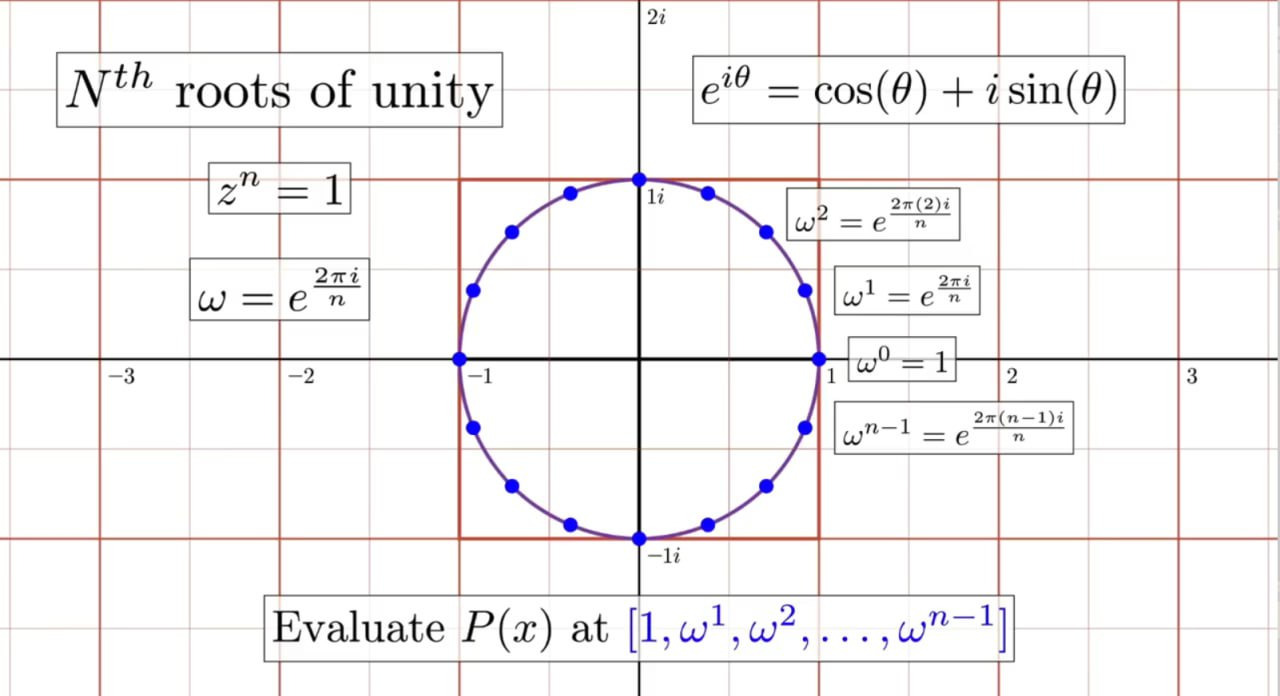
\includegraphics[width=1\textwidth]{Images/nthroot.jpg}
               
               \label{fig:enter-label}
               \end{figure}

              The polynomial $P(x)$ can equivalently be represented as the vector of coefficients $(p_0, p_1, \dots, p_{n-1})$. The Discrete Fourier Transform of the polynomial is defined as the values of the polynomial at the points $x = w_{k}$, i.e. it is the vector: \\

                \begin{align*} \text{DFT}(p_0, p_1, \dots, p_{n-1}) &= (y_0, y_1, \dots, y_{n-1}) \\ &= (P(w_{0}), P(w_{1}), \dots, P(w_{n-1})) \\ &= (P(w^0), P(w^1), \dots, P(w^{n-1})) \end{align*}
                \pagebreak

            On the other hand,  the Inverse Discrete Fourier Transform is defined: The inverse DFT of values of the polynomial $(y_0, y_1, \dots, y_{n-1})$ are the coefficients of the polynomial $(p_0, p_1, \dots, p_{n-1})$.
            $$\text{InverseDFT}(y_0, y_1, \dots, y_{n-1}) = (p_0, p_1, \dots, p_{n-1})$$

            Thus by using the $n^{th}$ roots of unity we can find the DFT of a polynomial( DFT on coefficients ) and by the Inverse DFT (Inverse DFT on values ) we again can restore the original coefficients of the polynomial.
            \\
            
            For fast multiplication of two polynomials DFT and Inverse DFT can be used. First find the DFT of the two polynomials let say ( $M(x)$ and $N(x)$ ) and their DFTs are $ DFT(M)$ and $ DFT(N) $.\\
            

             If we multiply the vectors $\text{DFT}(M)$ and $\text{DFT}(N)$ - by multiplying each element of one vector by the corresponding element of the other vector - then we get nothing other than the DFT of the polynomial $\text{DFT}(M \cdot N)$:
            $$\text{DFT}(M \cdot N) = \text{DFT}(M) \cdot \text{DFT}(N)$$

            Here, on the right side multiplication of DFTs we mean the pairwise product of the vector elements. This can be computed in $O(n)$ time. Next we do Inverse DFT on the result\\
            $$M \cdot N = \text{InverseDFT}(\text{DFT}(M) \cdot \text{DFT}(N))$$

            If this calculation needs $O(n\log n)$ computational steps, then the overall time complexity of the algorithm will be $O(n\log n)$.
            
\section{Fast Fourier Transform}

Fast Fourier Transform(FFT) is the solution of the previous computational complexity problem. Applying FFT the complexity can be reduced to $O(n\log n)$.Basically this algorithm uses divide and conquer technique to resolve the issue.\\

Let's take a polynomial $P(x)$ of order is $n-1$, where $n$ is a power of 2.

 $$P(x) = p_0 + p_1x 
 + p_2x^2 + ... + p_{n-1}x^{n-1}$$\\
 
 We divide it into two smaller polynomials, the one containing only the coefficients of the even positions, and the one containing the coefficients of the odd positions:
  \begin{align*} P_o(x) &= p_0 x^0 + p_2 x^1 + \dots + p_{n-2} x^{\frac{n}{2}-1} \\ P_e(x) &= p_1 x^0 + p_3 x^1 + \dots + p_{n-1} x^{\frac{n}{2}-1} \end{align*}

  \pagebreak
  The polynomial can also be represented as:\\
  $$P(x) = P_o(x^2) + x P_e(x^2).$$

  
The polynomials $P_o$ and $P_e$ are only half as much coefficients as the polynomial $P$. If we can compute the $\text{DFT}(P)$ in linear time using $\text{DFT}(P_o)$ and $\text{DFT}(P_e)$, then we get the recurrence $T_{\text{DFT}}(n) = 2 T_{\text{DFT}}\left(\frac{n}{2}\right) + O(n)$ for the time complexity, which results in $T_{\text{DFT}}(n) = O(n \log n)$ by the master theorem.\\

Let's say we have already computed the $\left(y_k^o\right)_{k=0}^{n/2-1}$ = $DFT(P_o)$ and \\ $\left(y_k^e\right)_{k=0}^{n/2-1}$ =$DFT(P_e)$\\ 

For the first $\frac{n}{2}$ values we can just use the previously noted equation\\ $P(x) = P_o(x^2) + x P_e(x^2)$:
$$y_k = y_k^o + w^k y_k^e, \quad k = 0,1, \dots ,\frac{n}{2} - 1.$$

The next $\frac{n}{2}$ values we need to find an expression which is pretty similar to our last expression of finding first half:
\begin{align*} y_{k+n/2} &= P\left(w^{k+n/2}\right) \\ &= P_o\left(w^{2k+n}\right) + w^{k + n/2} P_e\left(w^{2k+n}\right) \\ &= P_o\left(w^{2k} w^n\right) + w^k w^{n/2} P_e\left(w^{2k} w^n\right) \\ &= P_o\left(w^{2k}\right) - w^k P_e\left(w^{2k}\right) \\ &= y_k^o - w^k y_k^e \end{align*}






Here we used again $P(x) = P_o(x^2) + x P_e(x^2)$ and the two identities $w^n = 1$ and $w^{n/2} = -1$.

Therefore we get the desired formulas for computing the whole vector $(y_k)$:
\begin{align*} y_k &= y_k^o + w^k y_k^e, &\quad k = 0 \dots \frac{n}{2} - 1, \\ y_{k+n/2} &= y_k^o - w^k y_k^e, &\quad k = 0 \dots \frac{n}{2} - 1. \end{align*}

Thus we learned how to compute the DFT in $O(n \log n)$ time.



        
               
\end{document}

